%%%%%%%%%%%%%%%%%%%%%%%%%%%%%%%%%%%%%%%%%%%%%%%%%%%%%%%%%%%%%%%%%%%%%%%%%%%%%%%%
%% Projeto Final de Graduação
%% Aluno: Victor Seixas Souza
%% Orientadora: Christiane Neme Campos
%% Tema: Teoria de Ramsey em Grafos
%%%%%%%%%%%%%%%%%%%%%%%%%%%%%%%%%%%%%%%%%%%%%%%%%%%%%%%%%%%%%%%%%%%%%%%%%%%%%%%%
% !TEX root = ../thesis.tex
%%%%%%%%%%%%%%%%%%%%%%%%%%%%%%%%%%%%%%%%%%%%%%%%%%%%%%%%%%%%%%%%%%%%%%%%%%%%%%%%

\chapter{Método Probabilístico}
\label{chap:prob}

%%%%%%%%%%%%%%%%%%%%%%%%%%%%%%%%%%%%%%%%%%%%%%%%%%%%%%%%%%%%%%%%%%%%%%%%%%%%%%%%

O \indef{método probabilístico} é uma técnica não construtiva para demonstração da existência de objetos matemáticos com alguma propriedade específica. Como o próprio nome indica, o argumento tem natureza probabilística e consiste em mostrar que, ao escolher um objeto de maneira aleatória, a probabilidade deste objeto ter a propriedade desejada é positiva. Isto garante a existência deste objeto.

Cabe, então, antes de entra nos detalhes desta técnica, fazer uma breve revisão de conceitos de probabilidade, em particular, espaços discretos de probabilidade. Referências adicionais recomendadas incluem as notas de aula do Leonardo Rolla \cite{rolla} e o livro do Barry James \cite{barryjames}.

%%%%%%%%%%%%%%%%%%%%%%%%%%%%%%%%%%%%%%%%%%%%%%%%%%%%%%%%%%%%%%%%%%%%%%%%%%%%%%%%

\section{Probabilidade Discreta}

Para formalizar a probabilidade em matemática, introduzimos o conceito de um modelo probabilístico, que será o ambiente natural no qual podemos falar de probabilidade.
Um \indef{modelo probabilístico} possui três componentes básicas: um espaço amostral, uma classe de eventos e uma medida de probabilidade.

O \indef{espaço amostral} é um conjunto não vazio $\Omega$, cujos elementos representam os resultados possíveis para um experimento. Uma realização deste experimento consiste na escolha aleatória de um elemento $\omega \in \Omega$. Estamos interessados exclusivamente no caso em que $\Omega$ é um conjunto finito. Ao espaço amostral $\Omega$, associa-se uma classe $\mathcal{F}$ apropriada de subconjuntos de $Omega$. Os elementos de $\mathcal{F}$ são subconjuntos $A \subseteq \Omega$ aos quais atribuímos uma probabilidade, e são denominados \indef{eventos} ou \indef{conjuntos mensuráveis}. Definiremos probabilidade apenas para elementos desta classe. Para que isto seja feito de maneira adequada, a classe $\mathcal{F}$ precisa satisfazer algumas propriedades. Mais precisamente, $\mathcal{F}$ precisa formar uma $\sigma$-álgebra sobre $\Omega$~\cite{barryjames}.
No entanto, esta formalidade é facilmente contornada no caso discreto, uma vez que o conjunto de todos os subconjuntos de $\Omega$ é uma $\sigma$-álgebra sobre $\Omega$ quando $\Omega$ é finito. O par $(\Omega, \mathcal{F})$ é dito um \indef{espaço mensurável}.

Finalmente, uma \indef{medida de probabilidade}, ou simplesmente \indef{probabilidade}, é uma medida sobre o espaço mensurável $(\Omega, \mathcal{F})$, ou seja, uma função $\prob : \mathcal{F} \to \mathbb{R}$ com as seguintes propriedades:

\begin{enumerate}[label=(P\arabic*),itemindent=*]
  \item $\prob(A) \geq 0$ para todo $A \in \mathcal{F}$.
  \item $\prob(\Omega) = 1$.
  \item Se $A_1, A_2, \dots \in \mathcal{F}$ com $A_i \cap A_j = \emptyset, \forall i \neq j$, então $\prob( \bigcup_{i} A_i ) = \sum_i \prob(A_i)$.
\end{enumerate}

Um \indef{espaço de probabilidade} é uma tripla $(\Omega, \mathcal{F}, \prob)$ no qual $\Omega$ é um espaço amostral, $\mathcal{F}$ é uma classe de eventos e $\prob$ é uma medida de probabilidade sobre $(\Omega, \mathcal{F})$. Para um espaço de probabilidade, também valem as seguintes propriedades:

\begin{enumerate}[label=\arabic*.,itemindent=*]
  \item $\prob(\emptyset) = 0$;
  \item $\prob(\comp{A}) = 1 - \prob(A)$ onde $\comp{A} = \Omega \setminus A$;
  \item Se $A$ e $B \in \mathcal{F}$ e $A \subseteq B$, então $\prob(A) \leq \prob(B)$;
  \item Se $A$ e $B \in \mathcal{F}$ e $A \subseteq B$, então $\prob(B \setminus A) = \prob(B) - \prob(A)$;
  \item Para todo $A \in \mathcal{F}$, temos $0 \leq \prob(A) \leq 1$;
  \item Se $A_1, A_2, \dots \in \mathcal{F}$, então $\prob( \bigcup_{i} A_i ) \leq \sum_i \prob(A_i)$;
  \item Se $A$ e $B \in \mathcal{F}$, então $\prob(A \cup B) = \prob(A) + \prob(B) - \prob(A \cap B)$.
\end{enumerate}

Existem diversas maneiras de construir espaços de probabilidade, cada uma se adequando a uma situação. Para nossos propósitos, o espaço dos resultados \indef{equiprováveis} é de grande interesse e construído da seguinte maneira:
seja $\Omega$ um conjunto finito e $\mathcal{F}$ o conjunto de todos os subconjuntos de $\Omega$; para $A \in \mathcal{F}$, definimos a probabilidade de $A$ por $\prob(A) = \frac{\card{A}}{\card{\Omega}}$. Esta definição satisfaz as propriedades (P1), (P2) e (P3), portanto, é uma medida de probabilidade. Medidas de probabilidade sobre espaços finitos que satisfazem $\prob(A) = \frac{\card{A}}{\card{\Omega}}$ também são ditas \indef{uniformes}.

Dado um espaço de probabilidade $(\Omega, \mathcal{F}, \prob)$ e $A, B \in \mathcal{F}$, definimos a \indef{probabilidade condicional de $A$, dado que $B$ ocorre}, $\prob(A | B)$, por
\[ \prob(A|B) = \frac{\prob(A \cap B)}{\prob(B)}. \]
Quando $\prob(B) = 0$, definimos $\prob(A|B) = \prob(A)$. Desta forma, a função $\prob(\; \cdot \;| B) : \mathcal{F} \to \mathbb{R}$ é uma medida de probabilidade em $(\Omega, \mathcal{F})$ para qualquer $B \in \mathcal{F}$.

Dois eventos $A$ e $B$ são ditos \indef{independentes} se $\prob(A \cap B) = \prob(A) \cdot \prob(B)$. Intuitivamente, dois eventos são independentes quando a ocorrência ou não de um deles não influencia a probabilidade de ocorrência do outro evento.

\Needspace*{4\baselineskip}
As proposições a seguir são todas equivalentes.
\begin{enumerate}[label=\arabic*.,itemindent=*]
  \item $A$ e $B$ são independentes.
  \item $A$ e $\comp{B}$ são independentes.
  \item $\comp{A}$ e $B$ são independentes.
  \item $\comp{A}$ e $\comp{B}$ são independentes.
  \item $\prob(A|B) = \prob(A)$.
  \item $\prob(B|A) = \prob(B)$.
\end{enumerate}

Seja $\{ A_i : i \in I\}$ uma família de eventos, para a qual $I$ é um conjunto qualquer de índices. A família $\{ A_i : i \in I\}$ é dita \indef{independente dois a dois} se $A_i$ e $A_j$ são independentes para todo $i,j \in I$, $i \neq j$. A mesma família é dita \indef{mutuamente independente} se, para qualquer subconjunto $J \subset I$ de índices, vale
\[ \prob\left(\bigcap_{j \in J} A_j \right) = \prod_{j \in J}\prob(A_j).\]

Uma \indef{variável aleatória} é uma função $X: \Omega \to \mathbb{R}$ que associa a cada elemento do espaço amostral um valor real. Formalmente, também é requerido que o conjunto $\{ \omega \in \Omega : X(\omega) \leq x \}$ seja mensurável para todo $x$ real, ou seja, $X^{-1}( (-\infty,x]) \in \mathcal{F}$ para todo $x$. Quando $\Omega$ é finito e $\mathcal{F}$ é a classe de todos os subconjuntos de $\Omega$, este requisito sempre é satisfeito. Quando uma variável aleatória $X$ assume uma quantidade finita de valores, ela é dita \indef{simples}.

Utilizamos variáveis aleatórias para realizar contagens. Variáveis aleatórias que só assumem valores inteiros não negativos são chamadas de \indef{naturais}. Uma classe de variáveis aleatórias naturais bastante importante é a das \indef{funções indicadoras}. Fixado $A \subset \Omega$, definimos a função indicadora de $A$, $\ind{A}$, por
\[ \ind{A}(\omega) = \begin{cases}
  1, & \text{se } \omega \in A; \\
  0, & \text{se } \omega \not\in A.
\end{cases}\]

Dada uma variável aleatória natural $X$ sobre $(\Omega, \mathcal{F}, \prob)$, definimos a \indef{esperança} de $X$, denotada $\expec[X]$, por
\[ \expec[X] = \sum_{n = 0}^{\infty} n \prob(\{X = n\}).\]
Note que para funções indicadoras, temos $\expec[\ind{A}] = \prob(A)$.

A esperança é um operador \indef{linear} no seguinte sentido: sejam $X_1, \dots, X_n$ variáveis aleatórias sobre um mesmo espaço de probabilidade, e sejam $\alpha_1, \dots, \alpha_n \in \mathbb{R}$. Temos que
\[ \expec\left[ \sum_{i=1}^n \alpha_i X_i \right] = \sum_{i = 1}^{n} \alpha_i \expec[X_i]. \]

A esperança é \indef{monótona}, isto é, se $X$ e $Y$ são variáveis aleatórias em um mesmo espaço $\Omega$ com $X(\omega) \geq Y(\omega)$ para todo $\omega \in \Omega$, então $\expec[X] \geq \expec[Y]$.

A \indef{desigualdade de Markov} é uma importante ferramenta dentro do método probabilístico. Ela enuncia que se $X$ é uma variável aleatória não negativa, então
\[ \prob(X \geq a) \leq \frac{\expec[X]}{a}. \]

Este apanhado de resultados é suficiente para finalmente introduzirmos o método probabilístico aplicado em Teoria de Ramsey. Aplicações mais refinadas do método, no entanto, requerem conceitos mais avançados de probabilidade, como martingais, concentração de medida, grandes desvios e desigualdade de correlações. O livro \emph{The Probabilistic Method} \cite{alon} é a grande referência para o método e contém inúmeras aplicações tanto em Combinatória quanto em outras áreas da Matemática.

%%%%%%%%%%%%%%%%%%%%%%%%%%%%%%%%%%%%%%%%%%%%%%%%%%%%%%%%%%%%%%%%%%%%%%%%%%%%%%%%

\section{Limitantes Inferiores}

Os limitantes inferiores para os números de Ramsey vistos no Capítulo~\ref{chap:prelim} são construtivos, isto é, a demonstração de que $R(4,4) > 17$, por exemplo, passou pela construção de uma coloração de arestas do grafo $K_{17}$. Para encontrar bons limitantes inferiores de maneira mais genérica, precisamos de uma abordagem um pouco diferente. Vamos começar pelos números de Ramsey diagonais.

O nosso objetivo é encontrar colorações de arestas de $K_n$ sem $K_k$ monocromáticos com $k$ fixado e $n$ maior possível. Assim, podemos concluir que $R(k,k) > n$. Note que não precisamos necessariamente construir tal coloração, basta sabermos que alguma coloração que satisfaz estas propriedades existe. Vamos introduzir agora o \indef{método probabilístico} para resolver este tipo de problema. Para isso, queremos provar que uma estrutura com certas propriedades existe. Definimos, então, um espaço de probabilidade sobre o conjunto destas estruturas de maneira adequada e mostramos que, com probabilidade positiva, a propriedade de interesse é satisfeita. Isto nos mostra que o conjunto dos elementos cuja propriedade é satisfeita não pode ser vazio, caso contrário, a probabilidade seria zero, e mostramos a existência de uma estrutura com esta propriedade.

Esta técnica, embora aplicada pela primeira vez por Szele \cite{szele1943kombinatorikai}, foi vastamente explorada por Erdös, que utilizou esta técnica para encontrar justamente um limitante inferior para os números de Ramsey diagonais $R(k,k)$~\cite{erdos47}. Estamos interessados em escolher uma $RB$-coloração do $K_n$ de maneira aleatória e uniforme. O nosso espaço amostral $\Omega$ é, portanto, o conjunto de todas as colorações de arestas em duas cores do $K_n$. Seja $(\Omega, \mathcal{F}, \prob)$ o espaço de probabilidade com medida uniforme. Como temos que $|\Omega| = 2^{\binom{n}{2}}$, dado $A \in \mathcal{F}$, temos:
\[ \prob(A) = \frac{|A|}{2^{\binom{n}{2}}}.\]

Suponha que escolhemos uma coloração $c \in \Omega$ de maneira aleatória e uniforme, de acordo com o espaço de probabilidade acima. Queremos saber qual é a probabilidade desta coloração possuir uma dada propriedade. Seja $\mathcal{P} \subset \Omega$ o conjunto das colorações que satisfazem a dada propriedade. Temos, então, que $\prob(c \text{ possui a propriedade}) = \prob(c \in \mathcal{P}) = \card{\mathcal{P}} / \card{\Omega}$, onde $\prob$ é a medida de probabilidade.

Em particular, se $e$ é uma aresta, então $\card{\mathcal{P}} = \card{\{c \in \Omega : c(e) = R \}} = 2^{\binom{n}{2}-1}$, o que nos dá que $\prob(c(e) = R) = \frac{1}{2}$ e também que $\prob(c(e) = B) = \frac{1}{2}$.
Além disso, se $e$ e $f$ são arestas distintas, $\prob(c(e) = B \text{ e } c(f) = B) = \frac{1}{4}$, o que nos mostra que os eventos da forma $\{c(e) = C\}$ para alguma aresta $e$ e cor $C$ são independentes.

Desta forma, escolher uma coloração $c \in \Omega$ utilizando o espaço de probabilidade $(\Omega, \mathcal{F}, \prob)$ é equivalente a escolher uma coloração das arestas de $K_n$ colorindo cada aresta de maneira aleatória, uniforme e independente. Podemos agora introduzir a primeira aplicação do método probabilístico:

%%%%%%%%%%%%%%%%%%%%%%%%%%%%%%%%%%%%%%%%
\begin{theorem}[Erdös, 1947]
\label{thm:prob:method}
Se $\displaystyle \binom{n}{k} 2^{1 - \binom{k}{2}} < 1$ então $R(k,k) > n$. Isso nos dá que $R(k,k) > \lfloor 2^{k/2} \rfloor$ para todo $k \geq 3$.
\end{theorem}
%%%%%%%%%%%%%%%%%%%%%%%%%%%%%%%%%%%%%%%%
\begin{proof}
Suponha que $\binom{n}{k} 2^{1 - \binom{k}{2}} < 1$ e considere uma $RB$-coloração $c$ do grafo completo $G = (V,E) \iso K_n$ obtida pintando cada aresta de maneira aleatória, uniforme e independente. Fixado um subconjunto $A \in \binom{V}{k}$, ou seja, um subconjunto de $V$ com $k$ elementos, defina o evento $M_A = \{G[A] \text{ é monocromático em } c\}$.
Fixando uma cor para as arestas do subgrafo induzido por $A$, podemos colorir as demais $\binom{n}{2} - \binom{k}{2}$ arestas de qualquer cor. Como existem duas cores disponíveis, obtemos:
\[ \prob(M_A) = \frac{2\cdot 2^{\binom{n}{2} - \binom{k}{2}}}{2^{\binom{n}{2}}}  = 2^{1 - \binom{k}{2}}. \]

Considere agora a variável aleatória $X$, que conta a quantidade de $K_k$ monocromáticos em $K_n$. Temos então $X = \sum_{A \in \binom{V}{k}}\ind{M_A}$. Vamos calcular o valor esperado de $X$.

\begin{align*}
\expec[X] &= \expec\Bigg[\sum_{A \in \binom{V}{k}}\ind{M_A} \Bigg] = \sum_{A \in \binom{V}{k}} \expec[\ind{M_A}] \\
&= \sum_{A \in \binom{V}{k}} \prob(M_A) = \sum_{A \in \binom{V}{k}} 2^{1 - \binom{k}{2}}  = \binom{n}{k} 2^{1 - \binom{k}{2}} < 1.
\end{align*}

Pela desigualdade de Markov, $\prob(X \geq 1) \leq \expec[X] < 1$, logo $\prob(X = 0) > 0$. Portanto, existe alguma coloração de $K_n$ sem $K_k$ monocromático. Com isso, temos $R(k,k) > n$.

Lembre que $\binom{n}{k} \leq n^k /k!$ e suponha que $n = \lfloor 2^{k/2} \rfloor$. Temos, então, que
\[ \binom{n}{k}2^{1 - \binom{k}{2}} \leq \frac{n^k}{k!}2^{1 - \frac{k^2}{2} + \frac{k}{2}} = \frac{n^k 2^{1 + \frac{k}{2}}}{k!2^{\frac{k^2}{2}}} \leq \frac{2^{1 + \frac{k}{2}}}{k!} < 1, \]
quando $n \geq 3$. Assim, temos $R(k,k) > \lfloor 2^{k/2} \rfloor$ quando $n \geq 3$.
\end{proof}
%%%%%%%%%%%%%%%%%%%%%%%%%%%%%%%%%%%%%%%%

Este tipo de ideia pode ser refinado para obter resultados melhores para o limitante inferior. No entanto, não se conhece algum limitante inferior cuja ordem exponencial seja superior à $(\sqrt{2})^k$. Vimos anteriormente que o melhor limitante superior conhecido possui ordem exponencial $4^k$. Um dos problemas abertos mais importantes da Teoria de Ramsey é determinar a ordem exponencial correta para o crescimento dos números de Ramsey diagonais. Em particular, não se sabe se o seguinte limite existe~\cite{chung1983survey}:
\[ \lim_{k \to \infty} \left(R(k,k)  \right)^{1/k}. \]
Já mostramos que, se este limite existir, ele está entre $\sqrt{2}$ e $4$.

A diferença entre as ordens de crescimento do limitante inferior e do limitante superior nos mostra o quanto ainda não se sabe sobre estes números. O melhor que podemos fazer para encontrar um $K_k$ monocromático consiste em jogar fora metade do grafo a cada passo, como foi feito no Teorema~\ref{thm:intro:ramsey}, o que provavelmente é destrutivo demais. A melhor construção que encontramos para uma coloração sem $K_k$ monocromático é uma coloração aleatória. Toda construção explícita conhecida é sub-exponencial. De fato, um importante problema em aberto da Teoria de Ramsey é encontrar uma demonstração construtiva de que $R(k,k) \geq (1+c)^k$ para alguma constante $c > 0$.

Outro aspecto interessante desta demonstração é que ao alterar a desigualdade da condição de $\binom{n}{k} 2^{1 - \binom{k}{2}} < 1$ para $\binom{n}{k} 2^{1 - \binom{k}{2}} \ll 1$, garantimos que $\prob(X = 0) \to 1$. Com efeito, isso ocorre quando $n = \lfloor 2^{k/2} \rfloor$, o que possui implicações algorítmicas interessantes. Podemos encontrar, de fato, uma coloração do $K_n$ sem $K_{2\log n}$ monocromático com alta probabilidade apenas colorindo as arestas de maneira aleatória. Realmente, quanto maior $n$, menor a probabilidade de uma coloração aleatória do $K_n$ possuir um $K_{2\log n}$ monocromático.

%%%%%%%%%%%%%%%%%%%%%%%%%%%%%%%%%%%%%%%%%%%%%%%%%%%%%%%%%%%%%%%%%%%%%%%%%%%%%%%%

\section{Pequenas Alterações}

Na aplicação do método probabilístico da seção anterior, mostramos a existência de configurações em que alguma estrutura indesejada não ocorre. Algumas vezes, não conseguimos garantir que estas estruturas não apareçam, mas podemos encontrar configurações em que não existam muitas dessas estruturas ruins. O que podemos fazer, em seguida, é alterar esta configuração a fim de remover estas estruturas indesejadas. Este procedimento de realizar alterações nos grafos é bastante utilizado e geralmente permite refinar ligeiramente o nosso limitante inferior.

%%%%%%%%%%%%%%%%%%%%%%%%%%%%%%%%%%%%%%%%
\begin{theorem}
\label{thm:prob:alter}
Para todo inteiro $n$, temos $\displaystyle R(k,k) > n - \binom{n}{k}2^{1 - \binom{k}{2}}$.
\end{theorem}
%%%%%%%%%%%%%%%%%%%%%%%%%%%%%%%%%%%%%%%%
\begin{proof}
Considere uma $RB$-coloração $c$ do grafo completo com $n$ vértices obtida pintando cada aresta de maneira aleatória, uniforme e independente. Procedendo de maneira idêntica ao Teorema~\ref{thm:prob:method}, definimos a variável aleatória $X$ que conta a quantidade de $K_k$ monocromáticos no $K_n$. Calculamos o valor esperado de $X$ e obtivemos:
\[ \expec[X] = \binom{n}{k} 2^{1 - \binom{k}{2}}. \]

Isto é suficiente para garantir que existe uma coloração $c$ do $K_n$ com no máximo $\expec[X]$ cópias monocromáticas de $K_k$. Remova do $K_n$ um vértice de cada uma das cópias monocromáticas $K_k$ e, assim, obtemos um grafo livre de $K_k$ moncromático. Removemos no máximo $\expec[X]$ vértices e, assim, sobram pelo menos $n - \expec[X]$ vértices no grafo. Portanto
\[ R(k,k) \geq n - \expec[X] = n - \binom{n}{k} 2^{1 - \binom{k}{2}}.  \qedhere\]
\end{proof}
%%%%%%%%%%%%%%%%%%%%%%%%%%%%%%%%%%%%%%%%

J. Spencer~\cite{spencer2014asymptopia} fez uma análise cuidadosa desta desigualdade e obteve o resultado apresentado a seguir.

%%%%%%%%%%%%%%%%%%%%%%%%%%%%%%%%%%%%%%%%
\begin{noproofcorollary}
Para $k \to \infty$, temos $\displaystyle R(k,k) > (1+o(1))\frac{1}{e}k\sqrt{2}^k$.
\end{noproofcorollary}
%%%%%%%%%%%%%%%%%%%%%%%%%%%%%%%%%%%%%%%%

Até agora, vimos como utilizar o método probabilístico para encontrar limitantes para os números de Ramsey diagonais. Se desejarmos encontrar limitantes para outros números de Ramsey, precisamos alterar o nosso espaço de probabilidade.

Sejam $\Omega$ o conjunto de todas as $RB$-colorações do $K_n$ e $\mathcal{F}$ o conjunto de todos os subconjuntos de $\Omega$. Vamos construir uma medida de probabilidade que não é uniforme em $\Omega$. Fixe $0 \leq p \leq 1$ e pinte cada aresta de maneira aleatória e independente, com $\prob(c(e) = R) = p$ e $\prob(c(e) = B) = 1 - p$. Para uma coloração $c \in \Omega$ qualquer, temos
\[ \prob(c) =  p^{e(G_R)}(1-p)^{e(G_B)}.\]
Assim, $(\Omega, \mathcal{F}, \prob)$ forma um espaço de probabilidade. O espaço uniforme que tínhamos antes é o caso particular em que $p = 1/2$. Podemos generalizar o Teorema~\ref{thm:prob:alter} para números $R(k,s)$ conforme estabele o Teorema~\ref{thm:prob:alter_off}.

%%%%%%%%%%%%%%%%%%%%%%%%%%%%%%%%%%%%%%%%
\begin{theorem}
\label{thm:prob:alter_off}
Para todo inteiro $n$ e $p \in [0,1]$, temos $\displaystyle R(k, s) > n - \binom{n}{k}p^{\binom{k}{2}} - \binom{n}{s}(1-p)^{\binom{s}{2}}$.
\end{theorem}
%%%%%%%%%%%%%%%%%%%%%%%%%%%%%%%%%%%%%%%%
\begin{proof}
Considere uma $RB$-coloração $c$ do grafo completo $G = (V,E) \iso K_n$ obtida pintando cada aresta de maneira aleatória e independente de forma que cada aresta é vermelha com probabilidade $p$ e azul com probabilidade $1-p$.
Definimos a variável aleatória $X$ como a quantidade de cópias vermelhas de $K_k$ em $c$ e $Y$ como a quantidade de cópias azuis de $K_s$ em $c$. Computando as esperanças de $X$ e $Y$, obtemos:
\begin{align*}
\expec[X] &= \binom{n}{k}p^{\binom{k}{2}}; \\
\expec[Y] &= \binom{n}{s}(1-p)^{\binom{s}{2}}.
\end{align*}

Consideramos um \indef{grafo proibido} como uma cópia vermelha de $K_k$ ou uma cópia azul de $K_s$. Defina $Z = X + Y$ como a quantidade de grafos proibidos. Note que $\expec[Z] = \expec[X] + \expec[Y]$. Existe, portanto, uma coloração $c$ de $K_n$ com no máximo $\expec[Z]$ grafos proibidos. Removendo do $K_n$ um vértice de cada um dos grafos proibidos, obtemos um grafo livre de $K_k$ vermelho e de $K_s$ azul. Removemos no máximo $\expec[Z]$ vértices. Logo, sobram pelo menos $n - \expec[Z] $ vértices no grafo. Portanto,
\[ R(k, s) > n - \binom{n}{k}p^{\binom{k}{2}} - \binom{n}{s}(1-p)^{\binom{s}{2}}.  \qedhere\]
\end{proof}
%%%%%%%%%%%%%%%%%%%%%%%%%%%%%%%%%%%%%%%%

Esta modificação do resultado nos permite obter limitantes inferiores para outras classes de números. Fazendo escolhas adequadas de $n$ e $p$ no Teorema~\ref{thm:prob:alter_off}, obtém-se os corolários a seguir.

%%%%%%%%%%%%%%%%%%%%%%%%%%%%%%%%%%%%%%%%
\begin{noproofcorollary}
O número de Ramsey $R(3,k)$ satisfaz $\displaystyle R(3,k) \geq  \Omega\left( \frac{k^{3/2}}{\log^{3/2} k}\right)$.
\end{noproofcorollary}
%%%%%%%%%%%%%%%%%%%%%%%%%%%%%%%%%%%%%%%%

%%%%%%%%%%%%%%%%%%%%%%%%%%%%%%%%%%%%%%%%
\begin{noproofcorollary}
O número de Ramsey $R(4,k)$ satisfaz $\displaystyle R(4,k) \geq  \Omega\left( \frac{k^2}{\log^2 k}\right)$.
\end{noproofcorollary}
%%%%%%%%%%%%%%%%%%%%%%%%%%%%%%%%%%%%%%%%

%%%%%%%%%%%%%%%%%%%%%%%%%%%%%%%%%%%%%%%%%%%%%%%%%%%%%%%%%%%%%%%%%%%%%%%%%%%%%%%%

\section{O Lema Local de Lovász}

%%%%%%%%%%%%%%%%%%%%%%%%%%%%%%%%%%%%%%%%%%%%%%%%%%%%%%%%%%%%%%%%%%%%%%%%%%%%%%%%

Nas aplicações do método probabilístico apresentadas até agora, mostramos a existência de um objeto com determinada propriedade provando que a probabilidade da sua existência é maior do que zero. Em todos os casos que vimos, nós ainda provamos algo mais forte, vimos que a probabilidade deste evento é bastante alta. Em alguns casos, no entanto, o evento de interesse possui probabilidade baixa, mas positiva. Para lidar com este cenário, precisamos de técnicas mais refinadas.

Suponha que o objeto que estamos gerando aleatoriamente seja o que queremos encontrar quando alguns eventos raros não ocorrem. Sejam $\{E_i; i = 1,\dots,n\}$ estes eventos. Desejamos provar que existe a possibilidade de esses eventos não ocorrerem simultaneamente, isto é,  $\prob(\bigcap_{i=1}^n \comp{E_i}) > 0$. Um caso bem simples em que obtemos probabilidades bem pequenas é quando os $n$ eventos são mutuamente independentes, cada um com probabilidade $0 \leq p<1$. A probabilidade de todos os eventos não acontecerem simultaneamente é $(1-p)^n > 0$, e fica bem pequena à medida que $n$ cresce. A técnica do \indef{Lema Local de Lovász} (LLL) nos permite obter um resultado similar para eventos que não são mutuamente independentes, mas possuem dependências fracas entre si.

Para enunciar o LLL, precisamos introduzir o conceito de digrafo simples, que generaliza ligeiramente o conceito de grafo. Um \indef{digrafo} é um par ordenado $(V(D), A(D))$, que consiste em um conjunto $V(D)$ de \indef{vértices} e um conjunto $A(D)$ de \indef{arcos}, disjunto de $V(D)$, acompanhado de uma função de incidência $\Psi_D$ que associa cada arco de $A(D)$ a um par ordenado de vértices de $V(D)$, não necessariamente distintos. Diferentemente das arestas em grafos, os arcos dos digrafos são ordenados e, portanto, sugerem uma orientação. Se $a \in A(D)$ e $\Psi_D(a) = (u,v)$ dizemos que $u$ se liga a $v$. Além disso, dizemos que $u$ é a \indef{cauda} de $a$ e $v$ é a \indef{cabeça} de $a$.

Analogamente ao grafo simples, \indef{digrafo simples} é um digrafo no qual não existem arcos paralelos, isto é, $a$ e $b$ distintos em $A(D)$ com $\Psi_D(a) = \Psi_D(b)$. Portanto, um arco pode ser unicamente identificado com um par de elementos em $V(D) \times V(D)$, e a função de incidência fica implícita. Assim, podemos definir um digrafo simples como um par $D = (V,A)$ tal que $A \subset V\times V$.

Uma definição central para o LLL é a de digrafo de dependência, que caracteriza a estrutura de dependência entre variáveis aleatórias. Sejam $E_1, \dots, E_n$ eventos em um espaço de probabilidade $(\Omega, \mathcal{F}, \prob)$. Um digrafo simples $D = (V,A)$ é dito um \indef{digrafo de dependência} dos eventos $E_1, \dots, E_n$ quando $V = \{1, \dots, n\}$ e o evento $E_i$ é mutuamente independente dos eventos no conjunto $\{ E_j : (i,j) \not\in A, j \neq i\}$.

Por exemplo, considere duas moedas justas lançadas independentemente com resultados cara ($H$) ou coroa ($T$). Considere os seguintes eventos:
\begin{align*}
  E_1 &= \{ (H,H) , (H,T) \} && \text{Cara no primeiro lançamento;}\\
  E_2 &= \{ (H,H) , (T,H) \} && \text{Cara no segundo lançamento;}\\
  E_3 &= \{ (H,H) , (T,T) \} && \text{Lançamentos iguais.}
\end{align*}

Note que todos esses eventos tem probabilidade $\prob(E_i) = 1/2$ e, se $i \neq j$, temos $\prob(E_i | E_j) = 1/2$. Portanto, os eventos $E_i$ e $E_j$ são independentes. Note também que para todo $i,j,k$ distintos, $\prob(E_i | E_j \cap E_k) = 1$, logo $E_i$ não é mutuamente independente de $E_j$ e $E_k$. Desta forma, o digrafo da Figura~\ref{prob:fig:ddigraph} é um digrafo de dependência para estes eventos.

%%%%%%%%%%%%%%%%%%%%%%%%%%%%%%%%%%%%%%%%
\begin{figure}[ht!]
\centering
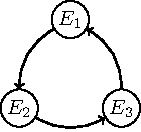
\includegraphics{figures/4_prob_1_ddigraph}
\caption{Um digrafo de dependência para os eventos $E_1$, $E_2$ e $E_3$.}
\label{prob:fig:ddigraph}
\end{figure}
%%%%%%%%%%%%%%%%%%%%%%%%%%%%%%%%%%%%%%%%

Note também que outras escolhas de arcos são possíveis para este mesmo exemplo. De fato, o digrafo apresentado na Figura~\ref{prob:fig:ddigraph2} também é um digrafo de dependência para os eventos $E_1$, $E_2$ e $E_3$, mostrando a não unicidade do digrafo de dependencia para um mesmo conjunto de eventos.

%%%%%%%%%%%%%%%%%%%%%%%%%%%%%%%%%%%%%%%%
\begin{figure}[ht!]
\centering
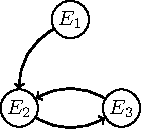
\includegraphics{figures/4_prob_2_ddigraph_2}
\caption{Outro digrafos de dependência para os mesmos eventos.}
\label{prob:fig:ddigraph2}
\end{figure}
%%%%%%%%%%%%%%%%%%%%%%%%%%%%%%%%%%%%%%%%

Podemos agora enunciar e demonstrar a versão geral do Lema Local de Lovász, que foi provado inicialmente por Erdös e Lovász~\cite{erdos1975problems}.

%%%%%%%%%%%%%%%%%%%%%%%%%%%%%%%%%%%%%%%%
\begin{lemma}[Lema Local de Lovász; Versão Geral]
\label{thm:prob:lll}
Sejam $E_1, \dots, E_n$ eventos em um espaço de probabilidade $(\Omega, \mathcal{F}, \prob)$. Suponha que $D = (V, A)$ seja um digrafo de dependência dos eventos $E_i$ e suponha que, para todo $1 \leq i \leq n$, existam números reais $x_1, \dotsc x_n$ tal que $0 \leq x_i < 1$ e $\prob (E_i) \leq x_i \prod_{(i,j) \in A}(1-x_j)$. Então
\[ \prob \left( \bigcap_{i = 1}^n \comp{E_i} \right) \geq \prod_{i = 1}^n (1 - x_i) > 0.\]
\end{lemma}
%%%%%%%%%%%%%%%%%%%%%%%%%%%%%%%%%%%%%%%%
\begin{proof}
Vamos mostrar por indução em $s$ que, para qualquer $S \subset \{1, \dots, n\}$ com $|S| = s < n$ e para todo $i \not\in S$, temos a seguinte desigualdade:
\[ \prob\bigg( E_i \bigg| \bigcap_{j \in S} \comp{E_j} \bigg) \leq x_i.\]

Para $s = 0$, não condicionamos em nenhum evento, logo $\prob(E_i) \leq x_i \prod_{(i,j) \in A}(1-x_j) \leq x_i$. Para o passo de indução, considere $S_1 = \{ j \in S : (i,j) \in A\}$ e $S_2 = \{ l \in S : (i,l) \not\in A \}$. Utilizando a definição de probabilidade condicional, obtemos
\begin{align*}
  \prob\bigg( E_i \bigg| \bigcap_{j \in S} \comp{E_j} \bigg) = \frac{\prob\left( E_i \cap \left(\bigcap_{j \in S_1} \comp{E_j} \right) \middle| \bigcap_{l \in S_2} \comp{E_l} \right)}{\prob\left( \bigcap_{j \in S_1} \comp{E_j} \middle| \bigcap_{l \in S_2} \comp{E_l} \right)}.
\end{align*}
Vamos agora limitar o numerador e o denominador individualmente. Para o numerador, note que o evento $E_i$ é mutuamente independente dos eventos $E_l$ com $l \in S_2$ pela definição de digrafo de dependência. Assim, temos:
\[ \prob\bigg( E_i \cap \bigg(\bigcap_{j \in S_1} \comp{E_j} \bigg) \bigg| \bigcap_{l \in S_2} \comp{E_l} \bigg) \leq \prob\bigg( E_i \bigg| \bigcap_{l \in S_2} \comp{E_l} \bigg) = \prob(E_i) \leq x_i \prod_{\mathclap{(i,j) \in A}}(1-x_j) \]

Já para o denominador, vamos utilizar a hipótese de indução. Suponha que $S_1 = \{j_1, j_2, \dots, j_r \}$. Se $r = 0$, então a interseção $\bigcap_{j \in \emptyset} \comp{E_j}  = \Omega$. Portanto, esta probabilidade é um e provamos a proposição apenas com o limitante do numerador. Com $r > 0$, obtemos:
\begin{align*}
&\prob \bigg( \comp{E_{j_1}} \cap \comp{E_{j_2}} \cap \dots \cap \comp{E_{j_r}} \bigg| \bigcap_{l \in S_2} \comp{E_l} \bigg) \\
=&\prob \bigg( \comp{E_{j_1}} \bigg| \bigcap_{l \in S_2} \comp{E_l} \bigg) \prob \bigg( \comp{E_{j_2}} \bigg| \comp{E_{j_1}} \cap \bigg(\bigcap_{l \in S_2} \comp{E_l} \bigg) \bigg) \cdots \prob \bigg( \comp{E_{j_r}} \bigg| \comp{E_{j_1}} \cap \dots \cap \comp{E_{j_{r-1}}} \cap \bigg(\bigcap_{l \in S_2} \comp{E_l}\bigg) \bigg) \\
\geq&(1-x_{j_1})(1-x_{j_2})\dots(1-x_{j_r}) \geq \prod_{\mathclap{(i,j) \in A}}(1-x_j).
\end{align*}

Portanto, obtemos
\begin{align*}
  \prob\bigg( E_i \bigg| \bigcap_{j \in S} \comp{E_j} \bigg) = \frac{\prob\left( E_i \cap \left(\bigcap_{j \in S_1} \comp{E_j} \right) \middle| \bigcap_{l \in S_2} \comp{E_l} \right)}{\prob\left( \bigcap_{j \in S_1} \comp{E_j} \middle| \bigcap_{l \in S_2} \comp{E_l} \right)} \leq \frac{x_i\prod_{(i,j) \in A}(1-x_j)}{\prod_{(i,j) \in A}(1-x_j)} = x_i.
\end{align*}

Finalmente, voltando ao enunciado original do lema, obtemos:
\begin{align*}
\prob \left( \bigcap_{i = 1}^n \comp{E_i} \right) &= \prob (\comp{E_1}) \prob (\comp{E_2} | \comp{E_1} ) \cdots \prob( \comp{E_n} | \comp{E_1} \cap \dots \cap \comp{E_{n-1}}) \\
&\geq (1 - x_1)(1 - x_2)\cdots(1-x_n) = \prod_{i=1}^n(1 - x_1) > 0. \qedhere
\end{align*}
\end{proof}
%%%%%%%%%%%%%%%%%%%%%%%%%%%%%%%%%%%%%%%%

Um caso particular de bastante interesse e mais fácil de aplicar é o chamado caso simétrico, que está enunciado em seguida.

%%%%%%%%%%%%%%%%%%%%%%%%%%%%%%%%%%%%%%%%
\begin{lemma}[Lema Local de Lovász; Versão Simétrica]
\label{thm:prob:llls}
Sejam $E_1, \dots, E_n$ eventos em um espaço de probabilidade $(\Omega, \mathcal{F}, \prob)$. Suponha que cada evento $E_i$ seja mutuamente independente de todos os outros eventos $E_j$ com no máximo $r$ exceções, e que $\prob(E_i) \leq p$ para todo $1 \leq i \leq n$. Se
\[ ep(r+1) \leq 1 \]
então $\prob \left( \bigcap_{i = 1}^n \comp{E_i} \right) > 0$. (A constante ``$e$'' da desigualdade acima é a constante de Euler.)
\end{lemma}
%%%%%%%%%%%%%%%%%%%%%%%%%%%%%%%%%%%%%%%%
\begin{proof}
Se $r = 0$, então $p < 1$ e os eventos são independentes. Caso contrário, construímos um digrafo de dependência $D = (V,A)$ para os eventos $E_1, \dots, E_n$ no qual, para cada $i$, $|\{j, (i,j) \in A\}| \leq r$. Escolhemos $x_i = \frac{1}{r+1}$ e vamos mostrar que $\prob (E_i) \leq x_i \prod_{(i,j) \in A}(1-x_j)$.
Com isso, satisfazemos as hipóteses do caso geral no Lema~\ref{thm:prob:lll} e, assim, concluímos que $\prob \left( \bigcap_{i = 1}^n \comp{E_i} \right) > 0$. De fato, lembrando que para todo $r$, $\frac{1}{e} < (1 - \frac{1}{r+1})^r$, temos
\[ \prob(E_i) \leq p \leq \frac{1}{e(r+1)} < \frac{1}{r+1}\left(1 - \frac{1}{r+1} \right)^r \leq x_i \prod_{\mathclap{(i,j) \in A}}(1-x_j). \qedhere\]
\end{proof}
%%%%%%%%%%%%%%%%%%%%%%%%%%%%%%%%%%%%%%%%

Foi mostrado por Shearer~\cite{shearer1985problem} que a constante ``$e$'' na desigualdade $ep(r+1) \leq 1$ é a melhor possível. Esta versão do Lema Local de Lovász possui diversas aplicações e produz bons resultados. De fato, o melhor limitante inferior conhecido para os números de Ramsey diagonais $R(k,k)$ é uma consequência desta versão do lema.

%%%%%%%%%%%%%%%%%%%%%%%%%%%%%%%%%%%%%%%%
\begin{theorem}[Spencer~\cite{spencer1975ramsey}]
\label{thm:prob:ramseylll}
Se $\displaystyle e \binom{k}{2}\binom{n-2}{k-2} 2^{1 - \binom{k}{2}} < 1$ então $R(k,k) > n$.
\end{theorem}
%%%%%%%%%%%%%%%%%%%%%%%%%%%%%%%%%%%%%%%%
\begin{proof}
Considere uma $RB$-coloração $c$ do grafo completo com $n$ vértices obtida pintando cada aresta de maneira aleatória, uniforme e independente. Fixado um subconjunto $A \in \binom{V}{k}$, defina o evento $M_A = \{G[A] \text{ é monocromático em } c\}$. Temos $\prob(M_A) = 2^{1- \binom{k}{2}}$. Se $S, T \subset V$ e $|S \cap T| \leq 1$, então os eventos $M_S$ e $M_T$ são independentes.
Além disso, se $|S \cap T| \geq 2$, então $M_S$ e $M_T$ são dependentes. Fixado $S$, vamos estimar a quantidade de conjuntos $T$ de $k$ vértices que satisfazem $|S \cap T| \geq 2$. Primeiramente, escolhemos dois vértices desta interseção, obtendo $\binom{k}{2}$ possibilidades. Os $k-2$ vértices restantes podem ser quaisquer vértices que não foram escolhidos anteriormente, o que implica em $\binom{n-2}{k-2}$ possibilidades. Desta forma, contamos mais de uma vez alguns conjuntos $T$, mas estimamos que no máximo $\binom{k}{2}\binom{n-2}{k-2}$ destes conjuntos existem.

Portanto, aplicando o Lema~\ref{thm:prob:llls} com $p = 2^{1 - \binom{k}{2}}$ e $r < \binom{k}{2}\binom{n-2}{k-2}$, e sabendo, por hipótese, que $ep(r+1) \leq 1$,
temos $\prob \left( \bigcap_{S \in \binom{V}{2}} \comp{M_S} \right) > 0$ e, assim, existe uma coloração de arestas de $K_n$ sem $K_k$ monocromáticos. Concluímos que $R(k,k) > n$.
\end{proof}
%%%%%%%%%%%%%%%%%%%%%%%%%%%%%%%%%%%%%%%%

Fazendo uma análise detalhada deste resultado e escolhendo $n$ de forma adequada, é possível obter que
\[R(k,k) > (1+o(1))\frac{\sqrt{2}}{e}k\sqrt{2}^k.\]
Este limitante inferior possui a constante ligeiramente melhor que o apresentado anteriormente; é o melhor limitante inferior conhecido para os números de Ramsey diagonais.

Uma análise similar pode ser feita para números de Ramsey não-diagonais, mas para isso, a versão geral do LLL é necessária. De fato, temos eventos de dois tipos, se $T \in \binom{V}{3}$, então definimos $A_T$ como o evento em que $T$ é um triângulo azul e, se $S \in \binom{V}{k}$, $B_S$ é o evento em que $S$ é um $K_k$ vermelho.
Temos $\prob(A_T) = p^3$ e $\prob(B_S) = (1-p)^{\binom{k}{2}}$.
Cada evento $A_T$ é dependente de no máximo $3(n-3) < 3n$ eventos $A_{T'}$ e $\binom{n}{k}$ eventos $B_{S'}$. Alem disso, cada evento $B_S$ é dependente de no máximo $\binom{k}{2}(n-2) < nk^2/2$ eventos $A_{T'}$ e $\binom{n}{k}$ eventos $B_{S'}$.
Segue, então, do Lema~\ref{thm:prob:lll}, que se existem $0 < p < 1$ e dois reais $0 \leq x,y < 1$, tais que
\begin{align*} p^3 \leq x(1-x)^{3n}(1-y)^{\binom{n}{k}} && \text{e} &&
(1-p)^{\binom{k}{2}} \leq y(1-x)^{nk^2/2}(1-y)^{\binom{n}{k}},
\end{align*}
temos que $R(3,k) > n$.

A melhor escolha possível para os parâmetros $p$, $x$ e $y$ é difícil de se encontrar, mas ela nos permite concluir que $R(3,k) > Ck^2/\log^2(k)$, para uma constante $C > 0$. A ordem de crescimento deste número foi determinada por Kim~\cite{kim1995ramsey}, que mostrou que
\[ R(3,k) = \Theta\left( \frac{k^2}{\log k}\right). \]
Determinar se existe uma constante $C$ tal que $R(3,k) \sim Ck^2 / \log k$ e determinar tal constante caso ela exista são dois problemas abertos fundamentais da Teoria de Ramsey.

A mesma ideia ainda pode ser utilizada para os números $R(4,k)$ e, em tal caso, encontramos que $R(4,k) > k^{5/2 + o(1)}$. Este limitante é melhor que qualquer outro limitante conhecido que pode ser provado sem utilizar o Lema Local de Lovász.

%%%%%%%%%%%%%%%%%%%%%%%%%%%%%%%%%%%%%%%%%%%%%%%%%%%%%%%%%%%%%%%%%%%%%%%%%%%%%%%%
